
\chapter{Proof techniques III --- Combinatorics}

{\em Tragedy is when I cut my finger. Comedy is when you fall into an open sewer and die. --Mel Brooks }

\section{Counting}
\label{sec:counting}

Many results in mathematics are answers to ``How many \ldots'' questions.

\noindent ``How many subsets does a finite set have?''

\noindent ``How many handshakes will transpire when $n$ people first meet?''

\noindent ``How many functions are there from a set of size $n$ to a set of size $m$?''

The title of this section, ``Counting,'' is not intended to evoke the usual
process of counting sheep, or counting change.  What we want is to be able
to count some collection \emph{in principle} so that we will be able to 
discover a formula for its size.

There are two principles that will be indispensable in counting things.
These principles are simple, yet powerful, and they have been named in
the most unimaginative way possible.  The ``multiplication rule'' which
tells us when we should multiply, and the ``addition rule'' which tells
us when we should add.  

Before we describe these principles in detail,
we'll have a look at a simpler problem which is most easily described
by an example: How many integers are there in the list $(7,8,9,\ldots 44)$?
We could certainly write down all the integers from $7$ to $44$ (inclusive) 
and then count them -- although this wouldn't be the best plan if the numbers
$7$ and $44$ were replaced with (say) $7,045,356$ and $22,355,201$.  A method
that does lead to a generalized ability to count the elements of a finite
sequence arises if we think carefully about what exactly a finite sequence 
\emph{is}.  

\begin{defi}
A \index{sequence}\emph{sequence from a set $S$} is a function from 
$\Naturals$ to $S$.
\end{defi}

\begin{defi}
A \index{finite sequence}\emph{finite sequence from a set $S$} is a 
function from $\{0, 1, 2, \ldots , n\}$ to $S$, where $n$ is some 
particular (finite) integer.  
\end{defi}

Now it is easy to see that there are $n+1$ elements in the set
$\{0, 1, 2, \ldots , n \}$ so counting the elements of a finite
sequence will be easy if we can determine the function involved 
and figure out what $n$ is by inverting it ($n$ is an inverse image
for the last element in a listing of the sequence). 

In the example that we started with, the function is $f(x)=x+7$.  We
can sum up the process that allows us to count the sequence by saying
``there is a one-to-one correspondence between the lists %

\[ (7, 8, 9, \ldots , 44 ) \]

\noindent and

\[ (0, 1, 2, \ldots , 37 ) \]

\noindent and the later has $38$ entries.''

More generally, if there is a list of consecutive numbers beginning
with $k$ and ending with $n$, there will be $n-k+1$ entries in the 
list.  Lists of consecutive integers represent a relatively simple
type of finite sequence.  Usually we would have some slightly more
interesting function that we'd need to invert.

The following exercise involves inverting the function $(x+5)^2$.


\begin{exer}
How many integers are in the list $(25, 36, 49, \ldots , 10000)$ ?
\end{exer}

We will have a lot more practice with counting the elements of sequences
in the exercises at the end of this section, let's continue on our
tour of counting by having a look at the addition rule.  

The \index{addition rule}addition rule says that it is appropriate to add if we can 
partition a collection into \emph{disjoint} pieces.  In other words,
if a set $S$ is the union of two or more subsets and these subsets 
are mutually disjoint, we can find the size of $S$ by adding the sizes
of the subsets.

In the game \index{Yahtzee}Yahtzee, one rolls 5 dice and (optionally) performs a 
second roll of some or all of the dice.  The object is to achieve 
several final configurations that are modeled after the hands in
Poker.  In particular, one configuration, known as a ``full house,''
is achieved by having two of one number and three of another. 
(Colloquially, we say ``three-of-a-kind plus a pair is a full house.'')

Now, we could use Yahtzee ``hands'' to provide us with a whole collection
of counting problems once we have our basic counting principles,
but for the moment we just want to make a simple (and obvious) point
about ``full houses'' -- the pair is either smaller or larger than
the three-of-a-kind.  This means we can partition the set of all possible
full houses into two disjoint sets -- the full houses consisting of a small
pair and a larger three-of-a-kind and those where the pair is larger 
than the three-of-a-kind.  If we can find some way of counting these
two cases separately, then the total number of full houses will be the 
sum of these numbers.

\begin{figure}[!hbtp]
\begin{center}
\begin{picture}(0,0)%
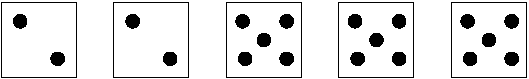
\includegraphics{./full_house_w_small_pair.pdf}%
\end{picture}%
\setlength{\unitlength}{3947sp}%
%
\begingroup\makeatletter\ifx\SetFigFont\undefined%
\gdef\SetFigFont#1#2#3#4#5{%
  \reset@font\fontsize{#1}{#2pt}%
  \fontfamily{#3}\fontseries{#4}\fontshape{#5}%
  \selectfont}%
\fi\endgroup%
\begin{picture}(4224,624)(1189,-973)
\end{picture}%


\vspace{.3in}

\begin{picture}(0,0)%
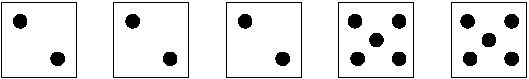
\includegraphics{./full_house_w_large_pair.pdf}%
\end{picture}%
\setlength{\unitlength}{3947sp}%
%
\begingroup\makeatletter\ifx\SetFigFont\undefined%
\gdef\SetFigFont#1#2#3#4#5{%
  \reset@font\fontsize{#1}{#2pt}%
  \fontfamily{#3}\fontseries{#4}\fontshape{#5}%
  \selectfont}%
\fi\endgroup%
\begin{picture}(4224,624)(1189,-973)
\end{picture}%

\end{center}
\caption[Full houses in Yahtzee.]{In Yahtzee, a full house may consist of 
a pair and a larger three-of-a-kind, or vice versa.}
\label{fig:full_house} 
\end{figure}


The \index{multiplication rule}multiplication rule gives 
us a way of counting things by thinking
about how we might construct them.  The numbers that are multiplied
are the number of choices we have in the construction process.  
Surprisingly often, the number of choices we can make in a given 
stage of constructing some configuration is independent of the choices
that have gone before -- if this is not the case the multiplication rule
may not apply.

If some object can be constructed in $k$ stages, and if in the first
stage we have $n_1$ choices as to how to proceed, in the second stage
we have $n_2$ choices, \emph{et cetera}.  Then the total number of such
objects is the product $n_1n_2 \cdots n_k$.

A \index{permutation}\emph{permutation of an $n$-set} (w.l.o.g. $\{1,2,\ldots , n\}$) is an ordered $n$-tuple where each entry is a distinct element of the
$n$-set.  Generally, a permutation may be regarded as a bijection from
an $n$-set to itself.  Our first use of the multiplication rule will
be to count the total number of permutations of $\{1, 2, 3, \ldots ,n\}$.

Let's start by counting the permutations of   $\{1, 2, 3\}$.  
A permutation will be a 3-tuple containing the numbers $1$, $2$ and
$3$ in some order.  We will think about building such a thing in 
three stages.  First,
we must select a number to go in the first position -- there are $3$ choices.
Having made that choice, there will only be two possibilities for the number
in the second position.  Finally there is just one number remaining to put in
the third position\footnote{People may say you have ``no choice'' in this %
last situation, but what they mean is that you have only one choice.}. 
Thus there are $3\cdot 2\cdot 1 = 6$ permutations of a $3$ element set.

The general rule is that there are $n!$ permutations of $\{1, 2, \ldots , n\}$.

There are times when configurations that are like permutations (in that they
are ordered and have no duplicates) but don't consist of all $n$ numbers 
are useful.  

\begin{defi}
A \emph{$k$-permutation from an $n$-set} is an ordered selection
of $k$ distinct elements from a set of size $n$.
\end{defi}

There are certain natural limitations on the value of $k$, for instance $k$
can't be negative -- although (arguably) $k$ can be 0, it makes more sense
to think of $k$ being at least 1.  Also, if $k$ exceeds
$n$ we won't be able to find \emph{any} $k$-permutations, 
since it will be impossible
to meet the ``distinct'' requirement.  If $k$ and $n$ are equal, there is 
no difference between a $k$-permutation and an ordinary permutation.  
Therefore, we ordinarily restrict $k$ to lie in the range $0 < k < n$.

The notation $P(n,k)$ is used for the total number of $k$-permutations
of a set of size $n$.  For example, $P(4,2)$ is 12, since there are
twelve different ordered pairs having distinct entries where the 
entries come from $\{1,2,3,4\}$.

\begin{exer}
Write down all twelve $2$-permutations of the $4$-set $\{1,2,3,4\}$.
\end{exer}

Counting $k$-permutations using the multiplication rule is easy.  We
build a $k$-permutation in $k$ stages.  In stage 1, we pick the first 
element in the permutation -- there are $n$ possible choices.  In
stage 2, we pick the second element -- there are now only $n-1$ choices
since we may not repeat the first entry.  We keep going like this until 
we've picked $k$ entries.  The number $P(n,k)$ is the product of $k$
numbers beginning with $n$ and descending down to $n-k+1$.  To verify 
that $n-k+1$ is really the right lower limit, check that there are indeed
$k$ entries in the sequence

\[ (n, n-1, n-2, \ldots n-k+1). \]

This verification may be easier if we rewrite the sequence as

\[ (n-0, n-1, n-2, \ldots n-(k-1) ). \]

Let's have a look at another small example -- $P(8,4)$.  There will be 8
choices for the first entry in a 4-tuple, 7 choices for the second
entry, 6 choices for the third entry and 5 choices for the last entry.
(Note that $5 = 8-4+1$.)  Thus $P(8,4)=8\cdot 7 \cdot 6 \cdot 5 = 1680$.

Finally, we should take note that it is relatively easy to express $P(n,k)$
using factorials.  If we divide a number factorialized by some smaller 
number factorialized, we will get a descending product just like those above.

\begin{exer}
What factorial would we divide $8!$ by in order to get $P(8,4)$?
\end{exer}

The general rule is that $P(n,k) = \frac{n!}{(n-k)!}$.

If we were playing a card game in which we were dealt 5 cards from
a deck of 52, we would receive our cards in the form of 
$P(52,5) = 52 \cdot 51 \cdot 50 \cdot 49 \cdot 48 = 311875200$ ordered
$5$-tuples.  Normally, we don't really care about what order the cards
came to us in.  In a card game one ordinarily begins sorting the cards
so as to see what hand one has -- this is a sure sign that the order the
cards were dealt is actually immaterial.  How many different orders can
five cards be put in?  The answer to this question is $5! = 120$ since
what we are discussing is nothing more than a permutation of a set of
size 5.  Thus, if we say that there are 311,875,200 different possible 
hands in 5-card poker, we are over-counting things by quite a bit!  Any
given hand will appear 120 times in that tabulation, which means the 
right value is $311875200/120 = 2598960$.  

Okay, so there around 2.6 million
different hands in 5-card poker.  Unless you plan to become a gambler
this isn't really that useful of a piece of information -- but if you
generalize what we've done in the paragraph above, you'll have found
a way to count unordered collections of a given size taken from a set.

A \index{combination} \emph{$k$-combination from an $n$-set} is an 
unordered selection, without repetitions, of $k$ things out of $n$.
This is the exact same thing as a subset of size $k$ of a set of size 
$n$, and the number of such things is denoted by several different 
notations -- $C(n,k)$, $nCk$ and $\displaystyle\binom{n}{k}$ among 
them\footnote{Watch out for the $\binom{n}{k}$ notation, it is easy 
to confuse it with the fraction $\left(\frac{n}{k}\right)$.  They are
not the same --- the fraction bar is \emph{supposed} to be missing
in $\binom{n}{k}$.}.  We can come
up with a formula for $C(n,k)$ by a slightly roundabout argument.
Suppose we think of counting the $k$-permutations of $n$ things using the
multiplication rule in a different way then we have previously.  We'll
build a $k$-permutation in two stages.  First we'll choose $k$ symbols
to put into our permutation -- which can be done in $C(n,k)$ ways.  And
second, we'll put those $k$ symbols into a particular order -- which
can be accomplished in $k!$ ways.  Thus $P(n,k) = C(n,k) \cdot k!$. 
Since we already know that $P(n,k) = \frac{n!}{(n-k)!}$, we can 
substitute and solve to obtain 

\[ C(n,k) = \frac{n!}{k! \cdot (n-k)!}. \]

It is possible to partition many counting problems into 4 ``types''
based on the answers to two questions:

Is order important in the configurations being counted?

Are we allowed to have repeated elements in a configuration?

Suppose that we are in the general situation of selecting $k$ things
out of a set of size $n$.  It should be possible to write formulas
involving $n$ and $k$ in the four cells of the following table.

\begin{center}
\begin{tabular}{cc}
 & Does order matter? \\
\parbox[c]{12pt}{ \begin{sideways} Are repeats okay? \end{sideways} }  & \begin{tabular}{c|c|c}
 & Yes & No \\ \hline
\parbox[c]{12pt}{ \begin{sideways} \rule{36pt}{0pt} No \end{sideways} } & \rule{0pt}{40pt}\rule{96pt}{0pt} & \rule{96pt}{0pt} \\ \hline
\parbox[c]{12pt}{ \begin{sideways} \rule{36pt}{0pt} Yes  \end{sideways} } & \rule{0pt}{40pt}\rule{96pt}{0pt} & \rule{96pt}{0pt} \\
\end{tabular}
\end{tabular}
\end{center}
\bigskip


\noindent{\bf Ordered with repetition}

Selecting a \index{PIN}PIN number\footnote{The phrase ``PIN number'' is 
redundant.  The `N' in PIN stands for ``number.''  Anyway, a PIN is
a four digit (secret) number used to help ensure that automated banking
(such as withdrawing your life's savings) is only done by an authorized
individual.}   for your bank account is a good example of
the kind of problem that is dealt with in the lower left part of the
table.  Obviously, the order in which you key-in the digits of your PIN
is important.  If one's number is 1356, it won't do to put in 6531!
Also there is no reason that we couldn't have repeated digits in a PIN.
(Although someone who chooses a PIN like 3333 is taking a bit of a security
risk!  A bad guy looking over your shoulder may easily discern what your
PIN is.)  A PIN is an ordered selection of 4 things out of 10, where 
repetition is allowed.  There are $10^4$ possible PINs.  We can determine
this by thinking of the multiplication principle -- there are 10 choices 
for the first digit of our PIN, since repetition is okay there are still
10 choices for our second digit, then (still) 10 choices for the third
digit as well as the fourth digit.

In general, when selecting $k$ things out of $n$ possibilities, where order
counts and repetition is allowed, there are $n^k$ possible selections.

\noindent{\bf Ordered without repetition}

Suppose that one wishes to come up with a password for a computer
account.  There are 52 letters (both upper and lower case) 10 numerals
and 32 symbols and punctuation marks -- for a total of 94 different 
characters that 
may be used.  Some system administrators can be very paranoid about
passwords that might be guessable -- for instance no password that 
appears in a dictionary should ever be used on a system where security
is a concern.  Suppose that your system administrator will reject any 
password that has repeated symbols, and that passwords must have 8 
characters.  How many passwords are possible?    

This is an instance of a counting problem where we are selecting 8 things
out of a set of size 94 -- clearly order is important and the system 
administrator's restriction means that we may not have repeats.
The multiplication rule tells us that there are 
$94\cdot 93\cdot 92\cdot 91\cdot 90\cdot 89\cdot 88\cdot 87 = 4488223369069440$
different passwords.  And in the general case (selecting $k$ things out 
of a set of size $n$, without repetition, and with order counting) 
there will be $n!/(n-k)!$ possibilities.  This is the number we have 
denoted previously by $P(n,k)$.

\noindent{\bf Unordered without repetition}

This is also a case that we've considered previously.  If we are choosing
$k$ things out of $n$ and order is unimportant and there can be no 
repetitions, then what we are describing is a $k$-subset of the 
$n$-set.  There are $C(n,k) = \frac{n!}{k!(n-k)!}$ distinct subsets.
Here, we'll give an example that doesn't sound like we're talking
about counting subsets of a particular size. (Although we really are!)

How many different sequences of 6 strictly increasing numbers can 
we choose from $\{1, 2, 3, \ldots 20\}$?  

Obviously, listing all such sequences would be an arduous task. 
We might start with $(1,2,3,4,5,6)$ and try to proceed in some 
orderly fashion to $(15,16,17,18,19,20)$, but unfortunately there
are 38,760 such sequences so unless we enlist the aid of a computer
we are unlikely to finish this job in a reasonable time.  The number
we've just given (38,760) is $C(20,6)$ and so it would seem that we're
claiming that this problem is really unordered selection without repetition
of 6 things out of 20.   Well, actually, some parts of this are clearly
right -- we are selecting 6 things from a set of size 20, and because
our sequences are supposed to be \emph{strictly} increasing there will 
be no repetitions -- but, a strictly increasing sequence is clearly 
\underline{ordered} and the formula we are using is for \underline{unordered}
collections.

By specifying a particular ordering (strictly increasing) on the sequences 
we are counting above, we are actually removing the importance of order.
Put another way: if order really mattered, the symbols $1$ through $6$
could be put into $720$ different orders -- but we only want to count 
one of those possibilities.  Put another other way: there is a one-to-one
correspondence between a $6$-subset of $\{1,2,3, \ldots 20\}$ and a
strictly increasing sequence.  Just make sure the subset is written in
increasing order!

Okay, at this point we have filled-in three out of the four cells in our table.

\begin{center}
\begin{tabular}{cc}
 & Does order matter? \\
\parbox[c]{12pt}{ \begin{sideways} Are repeats okay? \end{sideways} }  & \begin{tabular}{c|c|c}
 & \rule{108pt}{0pt} & \rule{108pt}{0pt} \\
 & Yes & No \\ \hline
\parbox[c]{12pt}{ \begin{sideways} \rule{36pt}{0pt} No \end{sideways} } & \rule{0pt}{60pt} \rule[-48pt]{0pt}{48pt} $P(n,k) = \frac{n!}{(n-k)!}$ & \rule{0pt}{60pt} \rule[-48pt]{0pt}{48pt}  $C(n,k) = \frac{n!}{k!(n-k)!}$ \\ \hline
\parbox[c]{12pt}{ \begin{sideways} \rule{36pt}{0pt} Yes  \end{sideways} } & \rule{0pt}{60pt} \rule[-48pt]{0pt}{48pt} $n^k$  & \rule{0pt}{60pt} \rule[-48pt]{0pt}{48pt}  \\
\end{tabular}
\end{tabular}
\end{center}

What kinds of things are we counting in the lower right part of the table?
Unordered selections of $k$ things out of $n$ possibilities where there may
(or may not!) be repetitions.  The game Yahtzee provides a nice example of
this type of configuration.  When we roll 5 dice, we do not do so 
one-at-a-time, rather, we roll them as a group -- the dice are 
indistinguishable so there is no way to order our set of 5 outcomes.
In fact, it would be quite reasonable to, after one's roll, arrange the
die in (say) increasing order.  We'll repeat a bit of advice that was given
previously: if one is free to rearrange a configuration to suit one's needs,
that is a clue that order is \emph{not} important in the configurations
under consideration.  Finally, are repetitions allowed?  The outcomes
in Yahtzee are 5 numbers from the set $\{1,2,3,4,5,6\}$, and while it
is possible to have no repetitions, that is a pretty special outcome!
In general, the same number can appear on two, or several, or even 
\emph{all 5} of the die\footnote{When this happens you are supposed 
to jump in the air and yell ``Yahtzee!''}.  

So, how many different outcomes
are there when one rolls five dice? To answer this question it will
be helpful to think about how we might express such an outcome.  
Since order is unimportant, we can choose to put the numbers that appear
on the individual die in whatever order we like.  We may as well place them
in increasing order.  There will be 5 numbers and each number is between 1
and 6.  We can list the outcomes systematically by starting with an all-ones
Yahtzee:

\begin{tabbing}
(1,1,1,1,1) \rule{8pt}{0pt} \= (1,1,1,1,2) \rule{8pt}{0pt} \= (1,1,1,1,3) \rule{8pt}{0pt} \= (1,1,1,1,4) \rule{8pt}{0pt} \= (1,1,1,1,5) \rule{8pt}{0pt} \= (1,1,1,1,6) \\ 
(1,1,1,2,2) \> (1,1,1,2,3) \> (1,1,1,2,4) \> (1,1,1,2,5) \> (1,1,1,2,6) \> (1,1,1,3,3) \\ 
(1,1,1,3,4) \> (1,1,1,3,5) \> (1,1,1,3,6) \> (1,1,1,4,4) \> (1,1,1,4,5) \> (1,1,1,4,6) \\ 
(1,1,1,5,5) \> (1,1,1,5,6) \> (1,1,1,6,6) \> (1,1,2,2,2) \> (1,1,2,2,3) \> (1,1,2,2,4) \\ 
(1,1,2,2,5) \> (1,1,2,2,6) \> (1,1,2,3,3) \> (1,1,2,3,4) \> (1,1,2,3,5) \> (1,1,2,3,6) \\ 
(1,1,2,4,4) \> (1,1,2,4,5) \> (1,1,2,4,6) \> (1,1,2,5,5) \> (1,1,2,5,6) \> (1,1,2,6,6) \\ 
(1,1,3,3,3) \> (1,1,3,3,4) \> (1,1,3,3,5) \> (1,1,3,3,6) \> (1,1,3,4,4) \> (1,1,3,4,5) \\ 
(1,1,3,4,6) \> (1,1,3,5,5) \> (1,1,3,5,6) \> (1,1,3,6,6) \> (1,1,4,4,4) \> (1,1,4,4,5) \\ 
(1,1,4,4,6) \> (1,1,4,5,5) \> (1,1,4,5,6) \> (1,1,4,6,6) \> (1,1,5,5,5) \> (1,1,5,5,6) \\ 
(1,1,5,6,6) \> (1,1,6,6,6) \> (1,2,2,2,2) \> (1,2,2,2,3) \> (1,2,2,2,4) \> (1,2,2,2,5) \\ 
(1,2,2,2,6) \> (1,2,2,3,3) \> (1,2,2,3,4) \> (1,2,2,3,5) \> (1,2,2,3,6) \> (1,2,2,4,4) \\ 
(1,2,2,4,5) \> (1,2,2,4,6) \> (1,2,2,5,5) \> (1,2,2,5,6) \> (1,2,2,6,6) \> (1,2,3,3,3) \\ 
(1,2,3,3,4) \> (1,2,3,3,5) \> (1,2,3,3,6) \> (1,2,3,4,4) \> (1,2,3,4,5) \> (1,2,3,4,6) \\ 
(1,2,3,5,5) \> (1,2,3,5,6) \> (1,2,3,6,6) \> (1,2,4,4,4) \> (1,2,4,4,5) \> (1,2,4,4,6) \\ 
(1,2,4,5,5) \> (1,2,4,5,6) \> (1,2,4,6,6) \> (1,2,5,5,5) \> (1,2,5,5,6) \> (1,2,5,6,6) \\ 
(1,2,6,6,6) \> (1,3,3,3,3) \> (1,3,3,3,4) \> (1,3,3,3,5) \> (1,3,3,3,6) \> (1,3,3,4,4) \\ 
(1,3,3,4,5) \> (1,3,3,4,6) \> (1,3,3,5,5) \> (1,3,3,5,6) \> (1,3,3,6,6) \> (1,3,4,4,4) \\ 
(1,3,4,4,5) \> (1,3,4,4,6) \> (1,3,4,5,5) \> (1,3,4,5,6) \> (1,3,4,6,6) \> (1,3,5,5,5) \\ 
(1,3,5,5,6) \> (1,3,5,6,6) \> (1,3,6,6,6) \> (1,4,4,4,4) \> (1,4,4,4,5) \> (1,4,4,4,6) \\ 
(1,4,4,5,5) \> (1,4,4,5,6) \> (1,4,4,6,6) \> (1,4,5,5,5) \> (1,4,5,5,6) \> (1,4,5,6,6) \\ 
(1,4,6,6,6) \> (1,5,5,5,5) \> (1,5,5,5,6) \> (1,5,5,6,6) \> (1,5,6,6,6) \> (1,6,6,6,6) \\ 
(2,2,2,2,2) \> (2,2,2,2,3) \> (2,2,2,2,4) \> (2,2,2,2,5) \> (2,2,2,2,6) \> (2,2,2,3,3) \\ 
(2,2,2,3,4) \> (2,2,2,3,5) \> (2,2,2,3,6) \> (2,2,2,4,4) \> (2,2,2,4,5) \> (2,2,2,4,6) \\ 
(2,2,2,5,5) \> (2,2,2,5,6) \> (2,2,2,6,6) \> (2,2,3,3,3) \> (2,2,3,3,4) \> (2,2,3,3,5) \\ 
(2,2,3,3,6) \> (2,2,3,4,4) \> (2,2,3,4,5) \> (2,2,3,4,6) \> (2,2,3,5,5) \> (2,2,3,5,6) \\ 
(2,2,3,6,6) \> (2,2,4,4,4) \> (2,2,4,4,5) \> (2,2,4,4,6) \> (2,2,4,5,5) \> (2,2,4,5,6) \\ 
(2,2,4,6,6) \> (2,2,5,5,5) \> (2,2,5,5,6) \> (2,2,5,6,6) \> (2,2,6,6,6) \> (2,3,3,3,3) \\ 
(2,3,3,3,4) \> (2,3,3,3,5) \> (2,3,3,3,6) \> (2,3,3,4,4) \> (2,3,3,4,5) \> (2,3,3,4,6) \\ 
(2,3,3,5,5) \> (2,3,3,5,6) \> (2,3,3,6,6) \> (2,3,4,4,4) \> (2,3,4,4,5) \> (2,3,4,4,6) \\ 
(2,3,4,5,5) \> (2,3,4,5,6) \> (2,3,4,6,6) \> (2,3,5,5,5) \> (2,3,5,5,6) \> (2,3,5,6,6) \\ 
(2,3,6,6,6) \> (2,4,4,4,4) \> (2,4,4,4,5) \> (2,4,4,4,6) \> (2,4,4,5,5) \> (2,4,4,5,6) \\ 
(2,4,4,6,6) \> (2,4,5,5,5) \> (2,4,5,5,6) \> (2,4,5,6,6) \> (2,4,6,6,6) \> (2,5,5,5,5) \\ 
(2,5,5,5,6) \> (2,5,5,6,6) \> (2,5,6,6,6) \> (2,6,6,6,6) \> (3,3,3,3,3) \> (3,3,3,3,4) \\ 
(3,3,3,3,5) \> (3,3,3,3,6) \> (3,3,3,4,4) \> (3,3,3,4,5) \> (3,3,3,4,6) \> (3,3,3,5,5) \\ 
(3,3,3,5,6) \> (3,3,3,6,6) \> (3,3,4,4,4) \> (3,3,4,4,5) \> (3,3,4,4,6) \> (3,3,4,5,5) \\ 
(3,3,4,5,6) \> (3,3,4,6,6) \> (3,3,5,5,5) \> (3,3,5,5,6) \> (3,3,5,6,6) \> (3,3,6,6,6) \\ 
(3,4,4,4,4) \> (3,4,4,4,5) \> (3,4,4,4,6) \> (3,4,4,5,5) \> (3,4,4,5,6) \> (3,4,4,6,6) \\ 
(3,4,5,5,5) \> (3,4,5,5,6) \> (3,4,5,6,6) \> (3,4,6,6,6) \> (3,5,5,5,5) \> (3,5,5,5,6) \\ 
(3,5,5,6,6) \> (3,5,6,6,6) \> (3,6,6,6,6) \> (4,4,4,4,4) \> (4,4,4,4,5) \> (4,4,4,4,6) \\ 
(4,4,4,5,5) \> (4,4,4,5,6) \> (4,4,4,6,6) \> (4,4,5,5,5) \> (4,4,5,5,6) \> (4,4,5,6,6) \\ 
(4,4,6,6,6) \> (4,5,5,5,5) \> (4,5,5,5,6) \> (4,5,5,6,6) \> (4,5,6,6,6) \> (4,6,6,6,6) \\ 
(5,5,5,5,5) \> (5,5,5,5,6) \> (5,5,5,6,6) \> (5,5,6,6,6) \> (5,6,6,6,6) \> (6,6,6,6,6) \\ 
\end{tabbing}

Whew \ldots err, I mean, Yahtzee!

You can describe a generic element of the above listing by saying ``It starts
with some number of 1's (which may be zero), then there are some 2's (again,
it might be that there are zero 2's),  then some (possibly none) 3's, 
then some 4's (or maybe not), then some
5's (I think you probably get the idea) and finally some 6's (sorry for 
all the parenthetical remarks).''  

We could, of course, actually count the 
outcomes as listed above (there are 252) but that would be pretty dull -- and
it wouldn't get us any closer to solving such problems in general.  To 
count things like Yahtzee rolls it will turn out that we can count something
related but much simpler -- blank-comma arrangements.  For the Yahtzee
problem we count arrangements of 5 blanks and 5 commas.  That is,
things like {\LARGE \blnk\blnk,\blnk,,\blnk,\blnk,} and 
{\LARGE \blnk\blnk\blnk\blnk\blnk,,,,,} and 
{\LARGE ,,,\blnk\blnk\blnk\blnk\blnk,,}.
These arrangements of blanks and commas correspond uniquely to Yahtzee
rolls -- the commas serve to separate different numerical values
and the blanks are where we would write-in the 5 outcomes on the die.


Convince yourself that there really is a one-to-one correspondence
between Yahtzee outcomes and arrangements of 5 blanks and 5 commas
by doing the following

\begin{exer}
What Yahtzee rolls correspond to the following blank-comma arrangements?

\noindent {\LARGE \blnk,\blnk,\blnk,\blnk,\blnk,} \hspace{\fill} {\LARGE \blnk\blnk,\blnk\blnk\blnk,,,,}  \hspace{\fill} {\LARGE ,,,,,\blnk\blnk\blnk\blnk\blnk}
\medskip

What blank-comma arrangements correspond to the following Yahtzee outcomes?

\noindent $\{2,3,4,5,6\}$  \hspace{\fill} $\{3,3,3,3,4\}$  \hspace{\fill} $\{5,5,6,6,6\}$

\end{exer}   

It may seem at first that this blank-comma thing is okay, but that we're 
still no closer to answering the question we started with.  It may seem
that way until you realize how easy it is to count these blank-comma
arrangements!  You see, there are 10 symbols in one of these blank-comma 
arrangements
and if we choose positions for (say) the commas, the blanks will have to go
into the other positions -- thus every 5-subset of $\{1,2,3,4,5,6,7,8,9,10\}$
gives us a blank-comma arrangement and every one of \emph{them} gives us
a Yahtzee outcome.  That is why there are $C(10, 5) = 252$ outcomes
listed in the giant tabulation above.

In general, when we are selecting $k$ things from a set of size $n$ 
(with repetition and without order) we will need to consider 
blank-comma arrangements having $k$ blanks and $n-1$ commas.  As an
aid to memory, consider that when you actually write-out the elements
of a set it takes one fewer commas than there are elements -- for example
$\{1,2,3,4\}$ has 4 elements but we only need 3 commas to separate them.
The general answer to our problem is either $C(k+n-1,k)$ or 
  $C(k+n-1, n-1)$, depending on whether you want to think about
selecting positions for the $k$ blanks or for the $n-1$ commas.  
It turns out that these binomial coefficients are equal so there's
no problem with the apparent ambiguity.

So, finally, our table of counting formulas is complete.  We'll produce
it here one more time and, while we're at it, ditch the $C(n,k)$ notation in 
favor of the more usual ``binomial coefficient'' notation $\binom{n}{k}$.

\begin{center}
\begin{tabular}{cc}
 & Does order matter? \\
\parbox[c]{12pt}{ \begin{sideways} Are repeats okay? \end{sideways} }  & \begin{tabular}{c|c|c}
 & \rule{108pt}{0pt} & \rule{108pt}{0pt} \\
 & Yes & No \\ \hline
\parbox[c]{12pt}{ \begin{sideways} \rule{36pt}{0pt} No \end{sideways} } & \rule{0pt}{60pt} \rule[-48pt]{0pt}{48pt} $P(n,k) = \frac{n!}{(n-k)!}$ & \rule{0pt}{60pt} \rule[-48pt]{0pt}{48pt}  $\binom{n}{k} = \frac{n!}{k!(n-k)!}$ \\ \hline
\parbox[c]{12pt}{ \begin{sideways} \rule{36pt}{0pt} Yes  \end{sideways} } & \rule{0pt}{60pt} \rule[-48pt]{0pt}{48pt} $n^k$  & \rule{0pt}{60pt} \rule[-48pt]{0pt}{48pt} 
$\binom{n+k-1}{k}$ \\
\end{tabular}
\end{tabular}
\end{center}

\clearpage

\noindent{\large \bf Exercises --- \thesection\ }

\begin{enumerate}
\item Determine the number of entries in the following sequences.

  \begin{enumerate}
  \item $(999, 1000, 1001, \ldots  2006)$
  \item $(13, 15, 17, \ldots 199)$
  \item $(13, 19, 25, \ldots 601)$
  \item $(5, 10, 17, 26, 37, \ldots 122)$
  \item $(27, 64, 125, 216, \ldots 8000)$
  \item $(7, 11, 19, 35, 67, \ldots 131075)$
  \end{enumerate}

\item How many ``full houses'' are there in Yahtzee?  (A full house is a pair
together with a three-of-a-kind.)

\item In how many ways can you get ``two pairs'' in Yahtzee?

\item Prove that the binomial coefficients $\displaystyle \binom{n+k-1}{k}$
and $\displaystyle \binom{n+k-1}{n-1}$ are equal.

\item The ``Cryptographer's alphabet'' is used to supply small examples
in coding and cryptography.  It consists of the first 6 letters, $\{a, b, c, d, e, f\}$.  How many ``words'' of length up to 6 can be made with this 
alphabet?  (A word need not actually be a word in English, for example 
both ``fed'' and ``dfe'' would be words in the sense we are using the term.)

\item How many ``words'' are there of length 4, with distinct letters from the 
Cryptographer's alphabet, in which the letters appear in increasing order 
alphabetically?  (``Acef'' would be one such word, but ``cafe'' would not.)

\item How many ``words'' are there of length 4 from the 
Cryptographer's alphabet, with repeated letters allowed,
 in which the letters appear in non-decreasing order alphabetically?


\item How many subsets does a finite set have?

\item How many handshakes will transpire when $n$ people first meet?

\item How many functions are there from a set of size $n$ to a set of size $m$?

\item How many relations are there from a set of size $n$ to a set of size $m$?

\end{enumerate}

%% Emacs customization
%% 
%% Local Variables: ***
%% TeX-master: "GIAM-hw.tex" ***
%% comment-column:0 ***
%% comment-start: "%% "  ***
%% comment-end:"***" ***
%% End: ***



\clearpage

\section{Parity and Counting arguments}

This section is concerned with two very powerful elements of the
proof-making arsenal: ``Parity'' is a way of referring to the result of
an even/odd calculation; Counting arguments most often take the form of
counting some collection in two different ways -- and then comparing
those results.  These techniques have little to do with one another,
but when they are applicable they tend to produce really elegant little
arguments.

In (very) early computers and business machines, paper cards were used to
store information.  A so-called \index{punch card}``punch card'' or 
\index{Hollerith card} ``Hollerith card'' was used to store 
binary information by means of holes punched into it.  Paper tape 
was also used in a similar fashion.  A typical paper tape format would
involve 8 positions in rows across the tape that might or might not be
punched, often a column of smaller holes would appear as well which 
did not store information but were used to drive the tape through the
reading mechanism on a sprocket.  Tapes and cards could be ``read'' either
by small sets of electrical contacts which would touch through a punched
hole or be kept separate if the position wasn't punched, or by using a
photo-detector to sense whether light could pass through the hole or not. 
The mechanisms for reading and writing on these paper media were amazingly
accurate, and allowed early data processing machines to use just a couple
of large file cabinets to store what now fits in a jump drive one can
wear on a necklace. (About 10 or 12 cabinets could hold a gigabyte
of data).  

Paper media was ideally suited to storing binary information, but of course
most of the real data people needed to store and process would be 
\index{alphanumeric}alphanumeric\footnote{``Alphanumeric'' is a somewhat
antiquated term that refers to information containing both alphabetic 
characters and numeric characters -- as well as punctuation marks, etc.}.
There were several encoding schemes that served to translate between the
character sets that people commonly used and the binary numerals that could
be stored on paper.  One of these schemes still survives today -- 
\index{ASCII}ASCII.
The American Standard Code for Information Interchange uses 7-bit binary
numerals to represent characters, so it contains 128 different symbols.
This is more than enough to represent both upper- and lower-case 
letters, the 10 numerals, and the punctuation marks -- many of the 
remaining spots in the ASCII code were used to contain so-called 
``control characters'' that were associated with functionality that
appeared on old-fashioned teletype equipment -- things like ``ring the bell,''
``move the carriage backwards one space,''  ``move the carriage 
to the next line,'' etc.   These control characters are why modern 
keyboards still have a modifier key labeled ``Ctrl'' on them.  The 
following listing gives the decimal and binary numerals from 0 to 127
and the ASCII characters associated with them -- the non-printing and
control characters have a 2 or 3 letter mnemonic designation.    
 
\renewcommand{\baselinestretch}{.9}
\renewcommand{\arraystretch}{.9}


\small \normalsize % A bogus font change is necessary to get LaTeX
                   % to take notice of the changed line spacing.

\begin{tabbing}
\rule{24pt}{0pt} \=0 \rule{24pt}{0pt} \=0000 0000  \rule{24pt}{0pt} \=\verb+NUL+  \rule{50pt}{0pt} \=64 \rule{24pt}{0pt} \=0100 0000 \rule{24pt}{0pt} \=\verb+@+  \\ 
\>1 \>0000 0001 \>\verb+SOH+   \>65 \>0100 0001 \>\verb+A+  \\ 
\>2 \>0000 0010 \>\verb+STX+   \>66 \>0100 0010 \>\verb+B+  \\ 
\>3 \>0000 0011 \>\verb+ETX+   \>67 \>0100 0011 \>\verb+C+  \\ 
\>4 \>0000 0100 \>\verb+EOT+   \>68 \>0100 0100 \>\verb+D+  \\ 
\>5 \>0000 0101 \>\verb+ENQ+   \>69 \>0100 0101 \>\verb+E+  \\ 
\>6 \>0000 0110 \>\verb+ACK+   \>70 \>0100 0110 \>\verb+F+  \\ 
\>7 \>0000 0111 \>\verb+BEL+   \>71 \>0100 0111 \>\verb+G+  \\ 
\>8 \>0000 1000 \>\verb+BS+    \>72 \>0100 1000 \>\verb+H+  \\ 
\>9 \>0000 1001 \>\verb+TAB+   \>73 \>0100 1001 \>\verb+I+  \\ 
\>10 \>0000 1010 \>\verb+LF+   \>74 \>0100 1010 \>\verb+J+  \\ 
\>11 \>0000 1011 \>\verb+VT+   \>75 \>0100 1011 \>\verb+K+  \\ 
\>12 \>0000 1100 \>\verb+FF+   \>76 \>0100 1100 \>\verb+L+  \\ 
\>13 \>0000 1101 \>\verb+CR+   \>77 \>0100 1101 \>\verb+M+  \\ 
\>14 \>0000 1110 \>\verb+SO+   \>78 \>0100 1110 \>\verb+N+  \\ 
\>15 \>0000 1111 \>\verb+SI+   \>79 \>0100 1111 \>\verb+O+  \\ 
\>16 \>0001 0000 \>\verb+DLE+  \>80 \>0101 0000 \>\verb+P+  \\ 
\>17 \>0001 0001 \>\verb+DC1+  \>81 \>0101 0001 \>\verb+Q+  \\ 
\>18 \>0001 0010 \>\verb+DC2+  \>82 \>0101 0010 \>\verb+R+  \\ 
\>19 \>0001 0011 \>\verb+DC3+  \>83 \>0101 0011 \>\verb+S+  \\ 
\>20 \>0001 0100 \>\verb+DC4+  \>84 \>0101 0100 \>\verb+T+  \\ 
\>21 \>0001 0101 \>\verb+NAK+  \>85 \>0101 0101 \>\verb+U+  \\ 
\>22 \>0001 0110 \>\verb+SYN+  \>86 \>0101 0110 \>\verb+V+  \\ 
\>23 \>0001 0111 \>\verb+ETB+  \>87 \>0101 0111 \>\verb+W+  \\ 
\>24 \>0001 1000 \>\verb+CAN+  \>88 \>0101 1000 \>\verb+X+  \\ 
\>25 \>0001 1001 \>\verb+EM+   \>89 \>0101 1001 \>\verb+Y+  \\ 
\>26 \>0001 1010 \>\verb+SUB+  \>90 \>0101 1010 \>\verb+Z+  \\ 
\>27 \>0001 1011 \>\verb+ESC+  \>91 \>0101 1011 \>\verb+[+  \\ 
\>28 \>0001 1100 \>\verb+FS+   \>92 \>0101 1100 \>\verb+\+  \\ 
\>29 \>0001 1101 \>\verb+GS+   \>93 \>0101 1101 \>\verb+]+  \\ 
\>30 \>0001 1110 \>\verb+RS+   \>94 \>0101 1110 \>\verb+^+  \\ 
\>31 \>0001 1111 \>\verb+US+   \>95 \>0101 1111 \>\verb+_+  \\ 
\>32 \>0010 0000 \>\verb+ +    \>96 \>0110 0000 \>\verb+`+  \\ 
\>33 \>0010 0001 \>\verb+!+    \>97 \>0110 0001 \>\verb+a+  \\ 
\>34 \>0010 0010 \>\verb+"+    \>98 \>0110 0010 \>\verb+b+  \\ 
\>35 \>0010 0011 \>\verb+#+    \>99 \>0110 0011 \>\verb+c+  \\ 
\>36 \>0010 0100 \>\verb+$+   \>100 \>0110 0100 \>\verb+d+  \\ 
\>37 \>0010 0101 \>\verb+%+   \>101 \>0110 0101 \>\verb+e+  \\ 
\>38 \>0010 0110 \>\verb+&+   \>102 \>0110 0110 \>\verb+f+  \\ 
\>39 \>0010 0111 \>\verb+'+   \>103 \>0110 0111 \>\verb+g+  \\ 
\>40 \>0010 1000 \>\verb+(+   \>104 \>0110 1000 \>\verb+h+  \\ 
\>41 \>0010 1001 \>\verb+)+   \>105 \>0110 1001 \>\verb+i+  \\ 
\>42 \>0010 1010 \>\verb+*+   \>106 \>0110 1010 \>\verb+j+  \\ 
\>43 \>0010 1011 \>\verb+++   \>107 \>0110 1011 \>\verb+k+  \\ 
\>44 \>0010 1100 \>\verb+,+   \>108 \>0110 1100 \>\verb+l+  \\ 
\>45 \>0010 1101 \>\verb+-+   \>109 \>0110 1101 \>\verb+m+  \\ 
\>46 \>0010 1110 \>\verb+.+   \>110 \>0110 1110 \>\verb+n+  \\ 
\>47 \>0010 1111 \>\verb+/+   \>111 \>0110 1111 \>\verb+o+  \\ 
\>48 \>0011 0000 \>\verb+0+   \>112 \>0111 0000 \>\verb+p+  \\ 
\>49 \>0011 0001 \>\verb+1+   \>113 \>0111 0001 \>\verb+q+  \\ 
\>50 \>0011 0010 \>\verb+2+   \>114 \>0111 0010 \>\verb+r+  \\ 
\>51 \>0011 0011 \>\verb+3+   \>115 \>0111 0011 \>\verb+s+  \\ 
\>52 \>0011 0100 \>\verb+4+   \>116 \>0111 0100 \>\verb+t+  \\ 
\>53 \>0011 0101 \>\verb+5+   \>117 \>0111 0101 \>\verb+u+  \\ 
\>54 \>0011 0110 \>\verb+6+   \>118 \>0111 0110 \>\verb+v+  \\ 
\>55 \>0011 0111 \>\verb+7+   \>119 \>0111 0111 \>\verb+w+  \\ 
\>56 \>0011 1000 \>\verb+8+   \>120 \>0111 1000 \>\verb+x+  \\ 
\>57 \>0011 1001 \>\verb+9+   \>121 \>0111 1001 \>\verb+y+  \\ 
\>58 \>0011 1010 \>\verb+:+   \>122 \>0111 1010 \>\verb+z+  \\ 
\>59 \>0011 1011 \>\verb+;+   \>123 \>0111 1011 \>\verb+{+  \\ 
\>60 \>0011 1100 \>\verb+<+   \>124 \>0111 1100 \>\verb+|+  \\ 
\>61 \>0011 1101 \>\verb+=+   \>125 \>0111 1101 \>\verb+}+  \\ 
\>62 \>0011 1110 \>\verb+>+   \>126 \>0111 1110 \>\verb+~+  \\ 
\>63 \>0011 1111 \>\verb+?+   \>127 \>0111 1111 \>\verb+DEL+  \\ 
\end{tabbing}

%A LaTeX comment containing a $ fixes format highliting.

\renewcommand{\baselinestretch}{1.3}
\renewcommand{\arraystretch}{.77}


\small \normalsize



Now it only takes 7 bits to encode the 128 possible values in the
ASCII system, which can easily be verified by noticing that the left-most
bits in all of the binary representations above are 0.   Most computers 
use 8 bit words or ``bytes'' as their basic units of information, and the
fact that the ASCII code only requires 7 bits lead someone to think up 
a use for that additional bit.  It became a ``parity check bit.''  If the
seven bits of an ASCII encoding have an odd number of 1's, the parity
check bit is set to 1 --- otherwise, it is set to 0.  The result of this
is that, subsequently, all of the 8 bit words that encode ASCII data will have
an even number of 1's.  This is an example of a so-called \index{error detecting code} error detecting
code known as the ``even code'' or the \index{parity check code}``parity check code.''  If 
data is sent over a noisy telecommunications channel, or is stored in
fallible computer memory, there is some small but calculable probability
that there will be a ``bit error.''   For instance, one computer might
send 10000111 (which is the ASCII code that says ``ring the bell'') but
another machine across the network might receive 10100111 (the 3rd bit from 
the left has been received in error) now if we are only looking at the 
rightmost seven bits we will think that the ASCII code for a single quote
has been received, but if we note that this piece of received data has an
odd number of ones we'll realize that something is amiss.  There are other
more advanced coding schemes that will let us not only \emph{detect} an
error, but (within limits) \emph{correct} it as well!  This rather amazing
feat is what makes wireless telephony (not to mention communications
with deep space probes --- whoops! I mentioned it) work.  

The concept of parity can be used in many settings to prove some
fairly remarkable results.  

In Section~\ref{sec:eq_rel} we introduced the idea of a graph.  This
notion was first used by \index{Euler, Leonhard} Leonhard Euler to solve
a recreational math problem posed by the citizens of 
\index{K\"{o}nigsberg}K\"{o}nigsberg, Prussia (this is the city now known
as \index{Kaliningrad} Kaliningrad, Russia.)  K\"{o}nigsberg was situated 
at a place where two branches of the \index{Pregel, Pregolya} Pregel river\footnote{Today, this river is known as the Pregolya.} come together -- there is also
a large island situated near this confluence.  By Euler's time, the city of
 K\"{o}nigsberg covered this island as well as the north and south banks of the
river and also the promontory where the branches came together.  A network of
seven bridges had been constructed to connect all these land masses.  The
townsfolk are alleged to have become enthralled by the question of whether it
was possible to leave one's home and take a walk through town
which crossed each of the bridges exactly once and, finally, return to one's
home.  

\begin{figure}[!hbtp]
\begin{center}
\begin{picture}(0,0)%
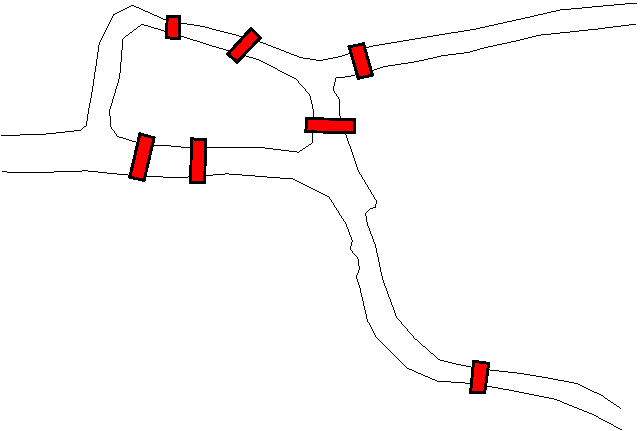
\includegraphics{./konigsberg.pdf}%
\end{picture}%
\setlength{\unitlength}{3947sp}%
%
\begingroup\makeatletter\ifx\SetFigFont\undefined%
\gdef\SetFigFont#1#2#3#4#5{%
  \reset@font\fontsize{#1}{#2pt}%
  \fontfamily{#3}\fontseries{#4}\fontshape{#5}%
  \selectfont}%
\fi\endgroup%
\begin{picture}(5111,3437)(152,-3280)
\end{picture}%

\end{center}
\caption[K\"{o}nigsberg, Prussia.]{A simplified map of K\"{o}nigsberg, Prussia
circa 1736.}
\label{fig:kon_map} 
\end{figure}

Euler settled the question (it can't be done) be converting the map of 
K\"{o}nigsberg into a graph and then making some simple observations about
the parities of the nodes in this graph.  The \index{degree} degree of a node
in a graph is the number of edges that are incident with it (if a so-called
``loop edge'' is present it adds two to the node's degree).  The ``parity
of a node'' is shorthand for the ``parity of the \emph{degree} of the node.'' 
 
\begin{figure}[!hbtp]
\begin{center}
\begin{picture}(0,0)%
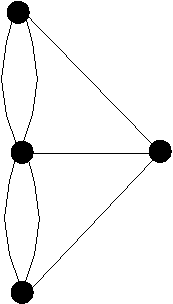
\includegraphics{figures/kon_graph.pdf}%
\end{picture}%
\setlength{\unitlength}{3947sp}%
%
\begingroup\makeatletter\ifx\SetFigFont\undefined%
\gdef\SetFigFont#1#2#3#4#5{%
  \reset@font\fontsize{#1}{#2pt}%
  \fontfamily{#3}\fontseries{#4}\fontshape{#5}%
  \selectfont}%
\fi\endgroup%
\begin{picture}(1377,2428)(2287,-3355)
\end{picture}%

\end{center}
\caption[K\"{o}nigsberg, Prussia as a graph.]{Euler's solution of the ``seven
bridges of K\"{o}nigsberg problem'' involved representing the town
as an undirected graph.}
\label{fig:kon_graph} 
\end{figure}

The graph of K\"{o}nigsberg has 4 nodes: one of degree 5 and three of degree
3.  All the nodes are odd.  Would it be possible to either modify 
K\"{o}nigsberg or come up with an entirely new graph having some even nodes?
Well, the answer to that is easy -- just tear down one of the bridges, and two
of the nodes will have their degree changed by one; they'll both become even.
Notice that, by removing one edge, we effected the parity of two nodes.  Is
it possible to create a graph with four nodes in which just one of them is
even?  More generally, given any short list of natural numbers, is it 
possible to draw a graph whose degrees are the listed numbers?

\begin{exer}
Try drawing graphs having the following lists of vertex degrees.
(In some cases it will be impossible\ldots)

\begin{itemize}
\item[-] $\{1,1,2,3,3\}$
\item[-] $\{1,2,3,5\}$
\item[-] $\{1,2,3,4\}$
\item[-] $\{4,4,4,4,5\}$
\item[-] $\{3,3,3,3\}$
\item[-] $\{3,3,3,3,3\}$
\end{itemize}
\end{exer}   
 
When it is possible to create a graph with a specified list
of vertex degrees, it is usually easy to do.  Of course, when 
it's impossible you struggle a bit\ldots \rule{5pt}{0pt} 
To help get things rolling (just in case you haven't
really done the exercise) I'll give a hint -- for the first list it 
is possible to draw a graph, for the second it is not.  
Can you distinguish the pattern?  What makes one list
of vertex degrees reasonable and another not?

\begin{exer}
(If you didn't do the last exercise, stop being such a lame-o and 
try it now.  BTW, if you \emph{did} do it, good for you!  You can
either join with me now in sneering at all those people who are scurrying
back to do the last one, or try the following:)  

Figure out a way to distinguish a sequence of numbers that \emph{can} be
the degree sequence of some graph from the sequences that cannot be.
\end{exer}

Okay, now if you're reading this sentence you should know that every 
other list of vertex degrees above is impossible, you should have graphs
drawn in the margin here for the 1st, 3rd and 5th degree sequences, and
you may have discovered some version of the following

\begin{thm} 
In an undirected graph, the number of vertices having an odd degree is even.
\end{thm}

A slightly pithier statement is: All graphs have an even number of 
odd nodes.

We'll leave the proof of this theorem to the exercises but most of the
work is done in proving the following equivalent result.

\begin{thm}
In an undirected graph the sum of the degrees of the vertices is even.
\end{thm}

\begin{proof}
The sum of the degrees of all the vertices in a graph $G$,

\[ \sum_{v\in V(G)} \deg(v), \]

\noindent counts every edge of $G$ exactly twice.

Thus,

 \[ \sum_{v\in V(G)} \deg(v) = 2 \cdot |E(G)|. \]

In particular we see that this sum is even.

\end{proof}

The question of whether a graph having a given list of vertex degrees
can exist comes down to an elegant little argument using both of the 
techniques in the title of this section.  We count the edge set of the 
graph in two ways -- once in the usual fashion and once by summing the 
vertex degrees; we also note that since this latter count is actually
a double count we can bring in the concept of parity.

 
Another perfectly lovely argument involving parity arises in questions
concerning whether or not it is possible to tile a pruned chessboard 
with dominoes.  We've seen dominoes before in Section~\ref{sec:induct}
and we're just hoping you've run across chessboards before.  Usually
a chessboard is 8 $\times$ 8, but we would like to adopt a more
liberal interpretation that a chessboard can be any rectangular grid
of squares we might choose.\footnote{The game known as ``draughts'' in the
UK and ``checkers'' in the US is played on an $8 \times 8$ board, but 
(for example) international draughts is played on a $10 \times 10$ 
board and Canadian checkers is played on a $12 \times 12$ board.}
Suppose that we have a supply of dominoes that are of just the right
size that if they are laid on a chessboard they perfectly cover two
adjacent squares.  Our first question is quite simple.  Is it possible
to perfectly tile an $m \times n$ chessboard with such dominoes? 

First let's specify the question a bit more.  By ``perfectly tiling''
a chessboard we mean that every domino lies (fully) on the board,
covering precisely two squares, and that every square of the board 
is covered by a domino.

The answer is straightforward.  If at least one of $m$ or $n$ is even
it can be done.  A necessary condition is that the number of squares
be even (since every domino covers two squares) and so, if both $m$ 
and $n$ are odd we will be out of luck.

A ``pruned board'' is obtained by either literally removing some of the
squares or perhaps by marking them as being off limits in some way.  
When we ask questions about perfect tilings of pruned chessboards things
get more interesting and the notion of parity can be used in several
ways.

Here are two tiling problems regarding square chessboards:


\begin{enumerate}
\item An even-sided square board (e.g. an ordinary $8 \times 8$ board) 
with diagonally opposite corners pruned.  
\item An odd-sided board with one square pruned.
\end{enumerate} 

Both of these situations satisfy the basic necessary condition that 
the number of squares on the board must be even.  You may be able
to determine another ``parity'' approach to these tiling problems
by attempting the following

\begin{exer}
Below are two five-by-five chessboards each having a single
square pruned.  One can be tiled by dominoes and the other
cannot.  Which is which?

 
\begin{center}
\begin{picture}(0,0)%
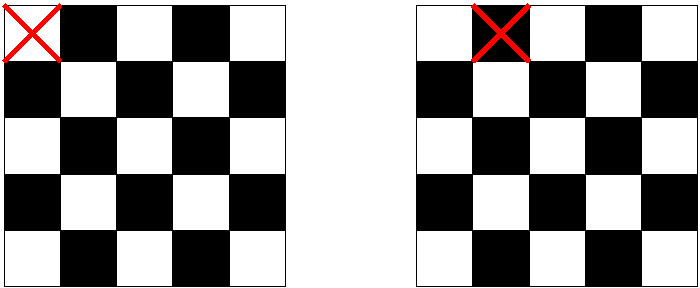
\includegraphics{./odd_pruned_chessboards.pdf}%
\end{picture}%
\setlength{\unitlength}{3947sp}%
%
\begingroup\makeatletter\ifx\SetFigFont\undefined%
\gdef\SetFigFont#1#2#3#4#5{%
  \reset@font\fontsize{#1}{#2pt}%
  \fontfamily{#3}\fontseries{#4}\fontshape{#5}%
  \selectfont}%
\fi\endgroup%
\begin{picture}(5595,2295)(868,-2248)
\end{picture}%

\end{center}

\end{exer}

The pattern of black and white squares on a chessboard is an 
example of a sort of artificial parity, if we number the squares
of the board appropriately then the odd squares will be white and
the even squares will be black.  We are used to chessboards having
this alternating black/white pattern on them, but nothing about these
tiling problems required that structure\footnote{Nothing about chess
requires this structure either, but it does let us do some error checking.
For instance, bishops always end up on the same color they left from and 
knights always switch colors as they move.}  If we were used to monochromatic chessboards, we might never solve the previous two problems -- unless
of course we invented the coloring scheme in order to solve them.  
An odd-by-odd chessboard has more squares of one color than of the other.
An odd-by-odd chessboard needs to have a square pruned in order for it to
be possible for it to be tiled by dominoes -- but if the wrong colored
square is pruned it will \emph{still} be impossible.  Each domino covers
two squares -- one of each color!  (So the pruned board must have the 
same number of white squares as black.) 

We'll close this section with another example of the technique of
counting in two ways.   

A \index{magic square} magic square of order $n$ is a square 
$n \times n$ array 
containing the numbers $1, 2, 3, \ldots , n^2$.  The numbers must 
be arranged in such a way that every row and every column sum to
the same number -- this value is known as the magic sum. 

For example, the following is an order $3$ magic square.

\begin{center}
\begin{tabular}{c|c|c}
\rule[-4pt]{0pt}{20pt}\rule{5pt}{0pt} 1 \rule{5pt}{0pt} & \rule{5pt}{0pt} 6 \rule{5pt}{0pt} & \rule{5pt}{0pt} 8 \rule{5pt}{0pt} \\ \hline
\rule[-4pt]{0pt}{20pt} 5 & 7 & 3 \\ \hline
\rule[-4pt]{0pt}{20pt} 9 & 2 & 4 \\
\end{tabular}
\end{center}

The definition of a magic square requires that the rows and columns sum to 
the same number but says nothing about what that number must be.  
It is conceivable that we could produce magic squares (of the same order)
having different magic sums.  This is \emph{conceivable}, but in fact the
magic sum is determined completely by $n$.

\begin{thm}
A magic square of order $n$ has a magic sum equal to $\displaystyle\frac{n^3+n}{2}$.
\end{thm}

\begin{proof}
We count the total of the entries in the magic square in two ways.
The sum of all the entries in the magic square is

\[ S = 1 + 2 + 3 + \ldots + n^2. \]

Using the formula for the sum of the first $k$ naturals ( $\sum_{i=1}^k i = \frac{k^2+k}{2}$) and evaluating at $n^2$ gives

\[ S = \frac{n^4 + n^2}{2}. \]

On the other hand, if the magic sum is $M$, then each of the $n$ rows has 
numbers in it which sum to $M$ so

\[ S = nM. \]

By equating these different expressions for $S$ and solving for $M$, we
prove the desired result:

\[ nM = \frac{n^4 + n^2}{2}, \]

\noindent therefore

\[ M = \frac{n^3 + n}{2}. \]

\end{proof} 

%Parity:
% Parity check bits and ``even'' codes.
% Graphs having certain lists of vertex degrees. (A graph must have an even 
%   number of odd vertices.)
% Covering a pruned chessboard with dominoes.
% Existance of an Eulerian circuit (or path) in a graph.
% The game of Nim.
% Why can't we make a 4x5 rectangle using the 5 tetrominoes?
%Counting:
% Magic squares.
% Block designs (bk=vr)
% R(3,3;2)

\clearpage

\noindent{\large \bf Exercises --- \thesection\ }


\begin{enumerate}

\item A walking tour of K\"{o}nigsberg such as is described in this section,
or more generally, a circuit through an arbitrary graph that crosses each
edge precisely once and begins and ends at the same node is known as
an \index{Eulerian circuit} \emph{Eulerian circuit}.  An \index{Eulerian
path} \emph{Eulerian path} also crosses every edge of a graph exactly
once but it begins and ends at distinct nodes.  For each of the following
graphs determine whether an Eulerian circuit or path is possible, and if so,
draw it.

\begin{center}
\begin{picture}(0,0)%
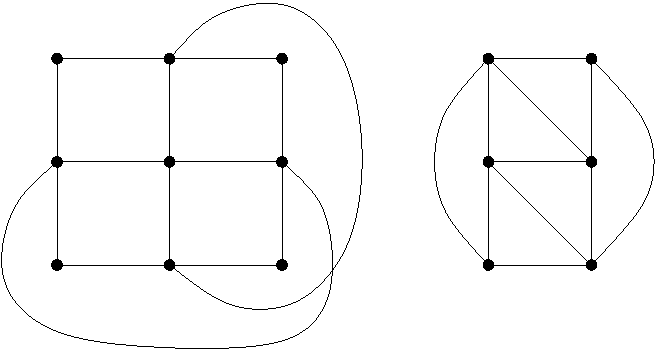
\includegraphics{./Euler_circuit_problems_a.pdf}%
\end{picture}%
\setlength{\unitlength}{3947sp}%
%
\begingroup\makeatletter\ifx\SetFigFont\undefined%
\gdef\SetFigFont#1#2#3#4#5{%
  \reset@font\fontsize{#1}{#2pt}%
  \fontfamily{#3}\fontseries{#4}\fontshape{#5}%
  \selectfont}%
\fi\endgroup%
\begin{picture}(5244,2786)(745,-2541)
\end{picture}%

\end{center}

\begin{center}
\begin{picture}(0,0)%
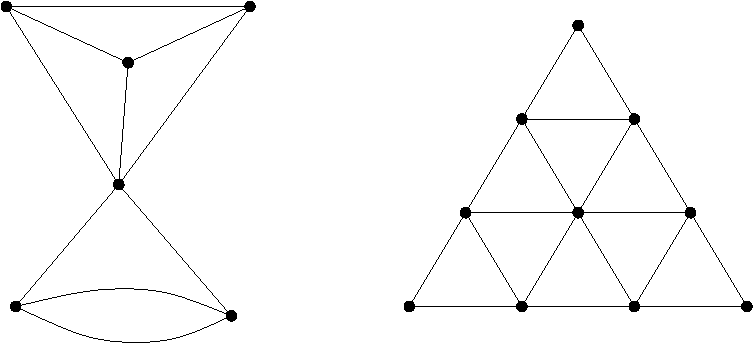
\includegraphics{./Euler_circuit_problems_b.pdf}%
\end{picture}%
\setlength{\unitlength}{3947sp}%
%
\begingroup\makeatletter\ifx\SetFigFont\undefined%
\gdef\SetFigFont#1#2#3#4#5{%
  \reset@font\fontsize{#1}{#2pt}%
  \fontfamily{#3}\fontseries{#4}\fontshape{#5}%
  \selectfont}%
\fi\endgroup%
\begin{picture}(6025,2749)(1226,-3136)
\end{picture}%

\end{center}

\item Complete the proof of the fact that ``Every graph has an even number
of odd nodes.''


\item Provide an argument as to why an $8 \times 8$ chessboard with 
two squares pruned from diagonally opposite corners cannot be tiled
with dominoes.

\item Prove that, if $n$ is odd, any $n \times n$ chessboard with 
a square the same color as one of its corners pruned can be tiled by
dominoes.

\item The five \index{tetromino} tetrominoes (familiar to players of the video game
Tetris) are relatives of dominoes made up of four small squares.

\begin{center}
\begin{picture}(0,0)%
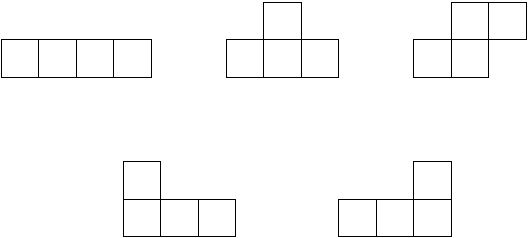
\includegraphics{figures/five_tetrominoes.pdf}%
\end{picture}%
\setlength{\unitlength}{3947sp}%
%
\begingroup\makeatletter\ifx\SetFigFont\undefined%
\gdef\SetFigFont#1#2#3#4#5{%
  \reset@font\fontsize{#1}{#2pt}%
  \fontfamily{#3}\fontseries{#4}\fontshape{#5}%
  \selectfont}%
\fi\endgroup%
\begin{picture}(4224,1899)(1189,-1948)
\end{picture}%

\end{center}

\noindent All together these five tetrominoes contain 20 squares
so it is conceivable that they could be used to tile a $4 \times 5$
chessboard.  Prove that this is actually impossible.

\item State necessary and sufficient conditions for the existence of
an Eulerian circuit in a graph.  

\item  State necessary and sufficient conditions for the existence of
an Eulerian path in a graph.  

\newpage

\item Construct magic squares of order 4 and 5.

\item A magic hexagon of order 2 would consist of filling-in
the numbers from 1 to 7 in the hexagonal array below.  The magic
condition means that each of the 9 ``lines'' of adjacent hexagons
would have the same sum.  Is this possible?

\begin{center}
\begin{picture}(0,0)%
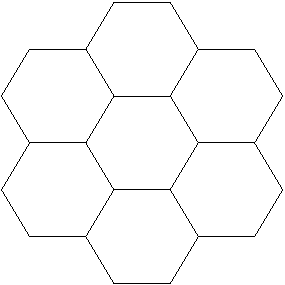
\includegraphics{figures/magic_hexagon.pdf}%
\end{picture}%
\setlength{\unitlength}{3947sp}%
%
\begingroup\makeatletter\ifx\SetFigFont\undefined%
\gdef\SetFigFont#1#2#3#4#5{%
  \reset@font\fontsize{#1}{#2pt}%
  \fontfamily{#3}\fontseries{#4}\fontshape{#5}%
  \selectfont}%
\fi\endgroup%
\begin{picture}(2274,2274)(2164,-3073)
\end{picture}%

\end{center}

\item Is there a magic hexagon of order 3?

\end{enumerate}



%% Emacs customization
%% 
%% Local Variables: ***
%% TeX-master: "GIAM-hw.tex" ***
%% comment-column:0 ***
%% comment-start: "%% "  ***
%% comment-end:"***" ***
%% End: ***



\clearpage


\section{The pigeonhole principle}

The word \index{pigeonhole} ``pigeonhole'' can refer to a hole in which a pigeon roosts
(i.e. pretty much what it sounds like) or a series of roughly square 
recesses in a desk in which one could sort correspondence (see Figure~\ref{fig:roll_top}).

\begin{figure}[!hbtp]
\begin{center}
\begin{picture}(0,0)%
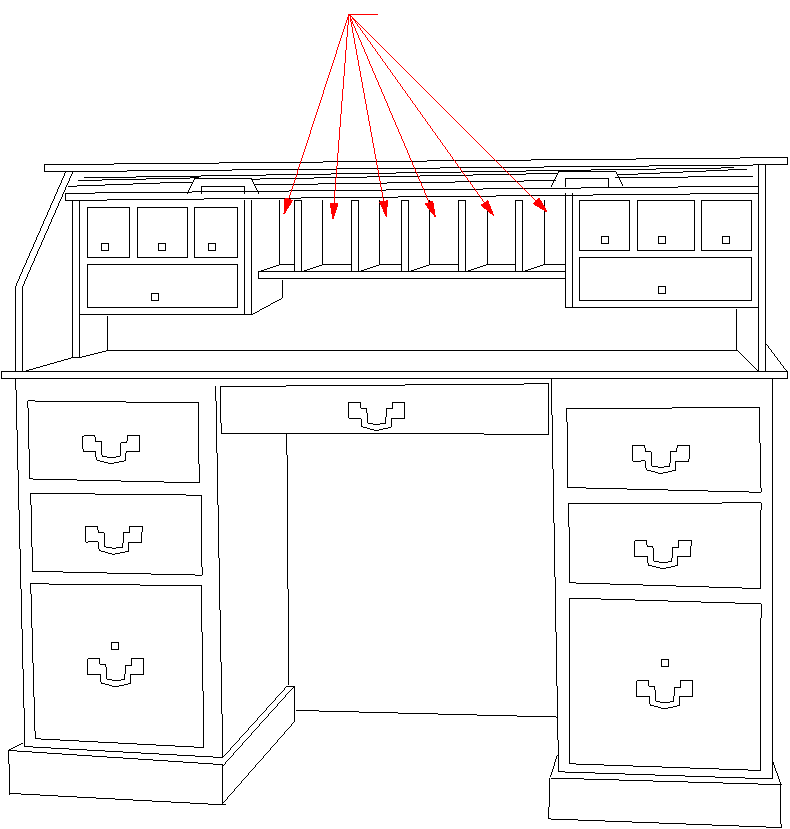
\includegraphics{figures/RollTopDesk.pdf}%
\end{picture}%
\setlength{\unitlength}{3947sp}%
%
\begingroup\makeatletter\ifx\SetFigFont\undefined%
\gdef\SetFigFont#1#2#3#4#5{%
  \reset@font\fontsize{#1}{#2pt}%
  \fontfamily{#3}\fontseries{#4}\fontshape{#5}%
  \selectfont}%
\fi\endgroup%
\begin{picture}(6309,6621)(1264,-6183)
\put(4388,279){\makebox(0,0)[lb]{\smash{{\SetFigFont{12}{14.4}{\rmdefault}{\mddefault}{\updefault}{\color[rgb]{0,0,0}pigeonholes}%
}}}}
\end{picture}%

\end{center}
\caption[A desk with pigeonholes.]{Pigeonholes in an old-fashioned roll top
desk could be used to sort letters.}
\label{fig:roll_top} 
\end{figure}

Whether you prefer to think of roosting birds or letters being sorted,
the first and easiest version of the \index{pigeonhole principle} pigeonhole principle is that if you
have more ``things'' than you have ``containers'' there must be a container
holding at least two things.

If we have 6 pigeons who are trying to roost in a coop with 5 pigeonholes,
two birds will have to share.

If we have 7 letters to sort and there are 6 pigeonholes in our desk, we
will have to put two letters in the same compartment.

The ``things'' and the ``containers'' don't necessarily have to be 
interpreted in the strict sense that the ``things'' go \emph{into} 
the ``containers.''
For instance, a nice application of the pigeonhole principle is that 
if there are at least 13 people present in a room, some pair of people 
will have been born in the same month.  In this example the things are the
people and the containers are the months of the year.

The abstract way to phrase the pigeonhole principle is:

\begin{thm}
If $f$ is a function such that $|\Dom{f}| > |\Rng{f}|$ then $f$ is not
injective.
\end{thm}

The proof of this statement is an easy example of proof by contradiction
so we'll include it here.

\begin{proof}
Suppose to the contrary that $f$ is a function with 
$|\Dom{f}| > |\Rng{f}|$ and that $f$ is injective.   Of course
$f$ is onto its range, so since we are presuming that $f$ is injective
it follows that $f$ is a bijection between $\Dom{f}$ and $\Rng{f}$.  Therefore (since $f$ provides a one-to-one
correspondence) $|\Dom{f}| = |\Rng{f}|$.  This clearly contradicts the
statement that $|\Dom{f}| > |\Rng{f}|$.
\end{proof}

For a statement with an almost trivial proof the pigeonhole principle
is very powerful.  We can use it to prove a host of existential 
results -- some are fairly silly, others very deep.  Here are a few 
examples:

There are two people (who are not bald) in New York City having exactly
the same number of hairs on their heads.

There are two books in (insert your favorite library) that have the 
same number of pages.

Given $n$ married couples (so $2n$ people) if we choose $n+1$ people
we will be forced to choose both members of some couple.

Suppose we select $n+1$ numbers from the set $\{1, 2, 3, \ldots, 2n\}$,
we will be forced to have chosen two numbers such that one is divisible 
by the other.  

\vspace{.25 in}

\centerline{\rule{108pt}{1pt}}

\vspace{.25 in}

We can come up with stronger forms of the pigeonhole principle by
considering pigeonholes with capacities.  Suppose we have 6 pigeonholes
in a desk, each of which can hold 10 letters.  What number of letters will
guarantee that one of the pigeonholes is full?  The largest number of letters
we could have without having 10 in some pigeonhole is $9 \cdot 6 = 54$, so if
there are 55 letters we must have 10 letters in some pigeonhole.

More generally, if we have $n$ containers, each capable of holding $m$
objects, than if there are $n \cdot (m-1) + 1$ objects placed in the 
containers, we will be assured that one of the containers is at capacity. 

The ordinary pigeonhole principle is the special case $m=2$ of this 
stronger version.

There is an even stronger version, which ordinarily is known as the 
\index{pigeonhole principle, strong form} ``strong form of the pigeonhole
principle.''  In the strong form, we have pigeonholes with an assortment
of capacities.

\begin{thm}
If there are $n$ containers having capacities $m_1, m_2, m_3, \ldots, m_n$,
and there are $1 + \sum_{i=1}^n (m_i - 1)$ objects placed in them, then for
some $i$, container $i$ has (at least) $m_i$ objects in it.
\end{thm} 

\begin{proof}
If no container holds its full capacity, then the largest the
total of the objects could be is $\sum_{i=1}^n (m_i - 1)$.
\end{proof}


\clearpage

\noindent{\large \bf Exercises --- \thesection\ }

\begin{enumerate}

\item The statement that there are two non-bald New Yorkers with
the same number of hairs on their heads requires some careful 
estimates to justify it.  Please justify it.

\item A mathematician, who always rises earlier than her spouse, has
developed a scheme -- using the pigeonhole principle -- to ensure that
she always has a matching pair of socks.  She keeps only blue socks, green 
socks and
black socks in her sock drawer -- 10 of each.  So as not to wake her 
husband she must
select some number of socks from her drawer in the early morning dark
and take them with her to the adjacent bathroom where she dresses.
What number of socks does she choose?

\item If we select $1001$ numbers from the set $\{1, 2, 3, \ldots, 2000\}$
it is certain that there will be two numbers selected such that one divides
the other.  We can prove this fact by noting that every number in the given
set can be expressed in the form $2^k \cdot m$ where $m$ is an odd number
and using the pigeonhole principle.  Write-up this proof.

\item Given any set of $53$ integers, show that there are two of them
having the property 
that either their sum or their difference is evenly divisible by $103$.

\item Prove that if $10$ points are placed inside a square of side length 3,
there will be 2 points within $\sqrt{2}$ of one another.

\item Prove that if $10$ points are placed inside an equilateral triangle
of side length 3, there will be 2 points within $1$ of one another.

\item Prove that in a simple graph (an undirected graph with no 
loops or parallel edges) having $n$ nodes, there must be two nodes 
having the same degree. 

\end{enumerate}


%% Emacs customization
%% 
%% Local Variables: ***
%% TeX-master: "GIAM-hw.tex" ***
%% comment-column:0 ***
%% comment-start: "%% "  ***
%% comment-end:"***" ***
%% End: ***



\clearpage

\section{The algebra of combinations}

Earlier in this chapter we determined the number of $k$-subsets of a set
of size $n$.  These numbers, denoted by $C(n,k) = nCk = \binom{n}{k}$
and determined by the formula $\frac{n!}{k!(n-k)!}$ are known as binomial 
coefficients.  It seems likely that you will have already seen the arrangement
of these binomial coefficients into a triangular array -- known as 
\index{Pascal's triangle} Pascal's triangle, but if not\ldots

\begin{center}
\begin{tabular}{ccccccccccccc}
  &   &   &   &    &    & 1  &    &    &   &   &   &   \\
  &   &   &   &    & 1  &    & 1  &    &   &   &   &   \\
  &   &   &   &  1 &    & 2  &    & 1  &   &   &   &   \\
  &   &   & 1 &    & 3  &    & 3  &    & 1 &   &   &   \\
  &   & 1 &   &  4 &    & 6  &    & 4  &   & 1 &   &   \\
  & 1 &   & 5 &    & 10 &    & 10 &    & 5 &   & 1 &   \\
1 &   & 6 &   & 15 &    & 20 &    & 15 &   & 6 &   & 1 \\
\end{tabular}
\end{center}

\noindent \emph{et cetera.}

The thing that makes this triangle so nice and that leads to the
strange name ``binomial coefficients'' for the number of $k$-combinations
of an $n$-set is that you can use the triangle to (very quickly) compute
powers of binomials.

A \index{binomial}\emph{binomial} is a polynomial with two terms.
Things like $(x+y)$, $(x+1)$ and $(x^7+x^3)$ all count as binomials
but to keep things simple just think about $(x+y)$.  If you need to
compute a large power of $(x+y)$ you can just multiply it out, for
example, think of finding the 6th power of $(x+y)$.

We can use the F.O.I.L rule to find $(x+y)^2 = x^2 + 2xy + y^2$. 
Then $(x+y)^3 =  (x+y) \cdot (x+y)^2 = (x+y) \cdot  (x^2 + 2xy + y^2)$.

You can compute that last product either by using the distributive law
or the table method:

\begin{center}
\begin{tabular}{c|ccc}
      & $x^2$ & $+ 2xy$ & $+ y^2$ \\ \hline
$x$   &       &         &         \\
$+ y$ &       &         &         \\
\end{tabular} 
\end{center}

Either way, the answer should be $(x+y)^3 = x^3 + 3x^2y + 3xy^2 + y^3$.

Finally the sixth power is the square of the cube thus

\begin{gather*} 
(x+y)^6 = (x+y)^3 \cdot (x+y)^3 \\
= (x^3 + 3x^2y + 3xy^2 + y^3) \cdot (x^3 + 3x^2y + 3xy^2 + y^3)
\end{gather*}

For this product I wouldn't even \emph{think} about the distributive
law, I'd jump to the table method right away:

\begin{center}
\begin{tabular}{r|cccc}
\rule[-6pt]{0pt}{24pt} & $x^3$ & $+ 3x^2y$ & $+ 3xy^2$ & $+ y^3$ \\ \hline
\rule[-6pt]{0pt}{24pt} $x^3$ & \rule{45pt}{0pt} & \rule{45pt}{0pt} & \rule{45pt}{0pt} & \rule{45pt}{0pt} \\
\rule[-6pt]{0pt}{24pt} $+ 3x^2y$ &       &           &           &         \\
\rule[-6pt]{0pt}{24pt} $+ 3xy^2$ &       &           &           &         \\
\rule[-6pt]{0pt}{24pt} $+ y^3$   &       &           &           &         \\

\end{tabular} 
\end{center}

In the end you should obtain 

\[ x^6 + 6 x^5y + 15 x^4y^2 + 20 x^3y^3 + 15 x^2y^4 + 6 xy^5 + y^6. \]

Now all of this is a lot of work and it's really much easier
to notice the form of the answer:  The exponent on $x$ starts at 6 and descends
with each successive term down to 0.  The exponent on $y$ starts at 0
and ascends to 6.  The coefficients in the answer are the numbers in the 
sixth row of Pascal's triangle.

Finally, the form of Pascal's triangle makes it really easy to extend.  
A number in the interior of the triangle is always the sum of the two
above it (on either side).  Numbers that aren't in the interior of the
triangle are always 1.


We showed rows 0 through 6 above.  Rows 7 and 8 are

\begin{center}
\begin{tabular}{ccccccccccccccccc}
   & 1 &   & 7 &    & 21 &    & 35 &    & 35 &    & 21 &    & 7 &   & 1 & \\
 1 &   & 8 &   & 28 &    & 56 &    & 70 &    & 56 &    & 28 &   & 8 &   & 1. \\ \end{tabular}
\end{center}

With this information in hand, it becomes nothing more than a matter of copying
down the answer to compute

\[ (x+y)^8 =  x^8 + 8x^7y + 28x^6y^2 + 56x^5y^3 + 70x^4y^4 + 56x^3y^5 + 28x^2y^6 + 8xy^7 + y^8. \]

\begin{exer} 
Given the method using Pascal's triangle for computing $(x+y)^n$ we can
use substitution to determine more general binomial powers.

Find $(x^4 + x^2)^5$.
\end{exer}

All of the above hinges on the fact that one can compute a binomial
coefficient by summing the two that appear to either side and above it
in Pascal's triangle.  This fact is the fundamental relationship
between binomial coefficients -- it is usually called Pascal's formula.

\begin{thm}
For all natural numbers $n$ and $k$ with $0 < k \leq n$,

\[ \binom{n}{k} = \binom{n-1}{k} + \binom{n-1}{k-1}. \]
\end{thm}

We are going to prove it twice.

\begin{proof} 
(The first proof is a combinatorial argument.)

There are $\binom{n}{k}$ subsets of size $k$ of the set $N = \{1, 2, 3, \ldots, n\}$.
We will partition these $k$-subsets into two disjoint cases: those that contain
the final number, $n$, and those that do not.

Let 

\[ A = \{ S \subseteq N \suchthat |S| = k \; \land \; n \notin S \} \]

\noindent and, let

\[ B = \{ S \subseteq N \suchthat |S| = k \; \land \; n \in S \}. \]

Since the number $n$ is either in a $k$-subset or it isn't, these sets
are disjoint and exhaustive.  So the addition rule tells us that

\[ \binom{n}{k} = |A| + |B|. \]

The set $A$ is really just the set of all $k$-subsets of the $(n-1)$-set
$\{1, 2, 3, \ldots, n-1 \}$, so $|A| = \binom{n-1}{k}$.

Any of the sets in $B$ can be obtained by adjoining the element $n$ to
a $k-1$ subset of the  $(n-1)$-set
$\{1, 2, 3, \ldots, n-1 \}$, so $|B| = \binom{n-1}{k-1}$.

Substituting gives us the desired result.
\end{proof}

\begin{proof}
(The second proof is algebraic in nature.)

Consider the sum 

\[ \binom{n-1}{k} + \binom{n-1}{k-1}.\]

Applying the formula we deduced in Section~\ref{sec:counting}
we get 

\begin{gather*} 
\binom{n-1}{k} + \binom{n-1}{k-1} \\
\rule{0pt}{36pt} = \frac{(n-1)!}{k! (n-1-k)!}  + \frac{(n-1)!}{(k-1)! ((n-1)-(k-1))!} \\
\rule{0pt}{36pt} = \frac{(n-1)!}{k! (n-k-1)!}  + \frac{(n-1)!}{(k-1)! (n-k)!} \\
\end{gather*}

A common denominator for these fractions is $k!(n-k)!$.  (We will have
to multiply the top and bottom of the first fraction by $(n-k)$ and the
top and bottom of the second fraction by $k$.)

\begin{gather*} 
= \frac{(n-k)(n-1)!}{k! (n-k) (n-k-1)!}  + \frac{k (n-1)!}{k (k-1)! (n-k)!} \\
\rule{0pt}{36pt} = \frac{(n-k)(n-1)!}{k! (n-k)!}  + \frac{k (n-1)!}{k! (n-k)!} \\
\rule{0pt}{36pt} = \frac{(n-k)(n-1)! + k (n-1)!}{k! (n-k)!} \\
\rule{0pt}{36pt} = \frac{(n-k+k)(n-1)!}{k! (n-k)!} \\
\rule{0pt}{36pt} = \frac{(n)(n-1)!}{k! (n-k)!} \\
\rule{0pt}{36pt} = \frac{n!}{k! (n-k)!}. \\
\end{gather*}


We recognize the final expression as the definition of $\binom{n}{k}$,
so we have proved that

\[ \binom{n-1}{k} + \binom{n-1}{k-1} = \binom{n}{k}. \]
\end{proof}

There are quite a few other identities concerning binomial coefficients
that can also be proved in (at least) two ways.  We will provide one
or two 
other examples and leave the rest to you in the exercises for this section.

\begin{thm}
For all natural numbers $n$ and $k$ with $0 < k \leq n$,

\[ k \cdot \binom{n}{k} = n \cdot \binom{n-1}{k-1}. \]
\end{thm}

Let's try a purely algebraic approach first.

\begin{proof}

Using the formula for the value of a binomial coefficient 
we get 

\[ k \cdot \binom{n}{k} = k \cdot \frac{n!}{k! (n-k)!}. \]

We can do some cancellation to obtain

\[ k \cdot \binom{n}{k} = \frac{n!}{(k-1)! (n-k)!}. \]

Finally we factor-out an $n$ to obtain

\[ k \cdot \binom{n}{k} = n \cdot \frac{(n-1)!}{(k-1)! (n-k)!}, \]

\noindent since $(n-k)$ is the same thing as $((n-1)-(k-1))$ we have

\[ k \cdot \binom{n}{k} = n \cdot \frac{(n-1)!}{(k-1)!((n-1)-(k-1))!} 
= n \cdot \binom{n-1}{k-1} \]

\end{proof}

A combinatorial argument usually involves counting \emph{something} 
in two ways.  What could that something be?  Well, if you see a 
product in some formula you should try to imagine what the 
multiplication rule would say in that particular circumstance.

\begin{proof} 
Consider the collection of all subsets of size $k$ taken from 
$N = \{1, 2, 3, \ldots, n\}$ in which one of the elements has
been marked to distinguish it from the others in some way.\footnote{
For example, a committee of $k$ individuals one of whom has been %
chosen as chairperson, is an example of the kind of entity we are %
discussing.}

We can count this collection in two ways using the multiplication rule.

Firstly, we could select a $k$-subset in $\binom{n}{k}$ ways and then from
among the $k$ elements of the subset we could select one to be marked.
By this analysis there are $\binom{n}{k} \cdot k$ elements in our
collection.

Secondly, we could select an element from the $n$-set which will be 
the ``marked'' element of our subset, and then choose the additional
$k-1$ elements from the remaining $n-1$ elements of the $n$-set.
By this analysis there are $n \cdot \binom{n-1}{k-1}$ elements in
the collection we have been discussing.

Thus,

\[ k \cdot \binom{n}{k} = n \cdot \binom{n-1}{k-1} \]

\end{proof}

The final result that we'll talk about actually has (at least) three proofs. 
One of which suffers from the fault that it is ``like swatting a fly
with a sledge hammer.''

The result concerns the sum of all the numbers in some 
row of Pascal's triangle.


\begin{thm}
For all natural numbers $n$ and $k$ with $0 < k \leq n$,

\[ \sum_{k=0}^n \binom{n}{k} = 2^n \]
\end{thm}

Our sledge hammer is a powerful result known as the binomial theorem
which is a formalized statement of the material we began this section
with. 

\begin{thm}[The Binomial Theorem]
For all natural numbers $n$, and real numbers $x$ and $y$, 

\[ (x+y)^n = \sum_{k=0}^{n} \binom{n}{k} x^{n-k}y^k. \] 
\end{thm}

We won't be proving this result just now.   But, the following proof
is a proof of the previous theorem using this more powerful result.

\begin{proof}
Substitute $x=y=1$ in the binomial theorem.
\end{proof} 

Our second proof will be combinatorial.
Let us re-iterate that a combinatorial proof usually consists of 
counting some collection in two different ways.  The formula
we have in this example contains a sum, so we should search for 
a collection of things that can be counted using the addition
rule.

\begin{proof} 
The set of all subsets of $N = \{1, 2, 3, \ldots, n\}$, which we
denote by ${\mathcal P}(N)$, can be partitioned into $n+1$ sets based
on the sizes of the subsets,

\[ {\mathcal P}(N) = S_0 \cup S_1 \cup S_2 \cup \ldots \cup S_n, \]

\noindent where $S_k = \{ S \suchthat S \subseteq N \; \land \; |S| = k \}$
for $0 \leq k \leq n$.  Since no subset of $N$ can appear in two different
parts of the partition (a subset's size is unique) and every subset of $N$
appears in one of the parts of the partition (the sizes of subsets are
all in the range from $0$ to $n$).  The addition principle tells us that

\[ |{\mathcal P}(N)| \quad = \quad |S_0| \;+\; |S_1| \;+\;\cup |S_2| \;+\; \ldots \;+\; |S_n|. \]

We have previously proved that $ |{\mathcal P}(N)| = 2^n$ and we know that
$|S_k| = \binom{n}{k}$ so it follows that


\[ 2^n = \binom{n}{0} + \binom{n}{1} +\binom{n}{2} + \ldots + \binom{n}{n}. \] 

\end{proof}

\clearpage

\noindent{\large \bf Exercises --- \thesection\ }

\begin{enumerate}

\item Use the binomial theorem (with $x=1000$ and $y=1$) to calculate
$1001^6$.

\item Find $(2x+3)^5$.

\item Find $(x^2+y^2)^6$.

\item The following diagram contains a 3-dimensional analog of
Pascal's triangle that we might call ``Pascal's tetrahedron.'' 
What would the next layer look like?

\begin{center}
\begin{picture}(0,0)%
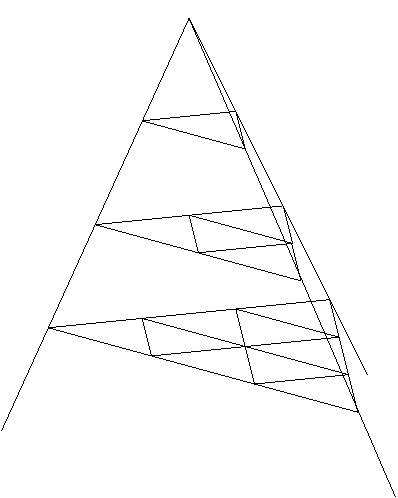
\includegraphics{figures/Pascals_tetrahedron.pdf}%
\end{picture}%
\setlength{\unitlength}{3947sp}%
%
\begingroup\makeatletter\ifx\SetFigFont\undefined%
\gdef\SetFigFont#1#2#3#4#5{%
  \reset@font\fontsize{#1}{#2pt}%
  \fontfamily{#3}\fontseries{#4}\fontshape{#5}%
  \selectfont}%
\fi\endgroup%
\begin{picture}(3174,3971)(3889,-4123)
\put(4876,-1111){\makebox(0,0)[lb]{\smash{{\SetFigFont{12}{14.4}{\familydefault}{\mddefault}{\updefault}{\color[rgb]{0,0,0}$1$}%
}}}}
\put(5851,-1036){\makebox(0,0)[lb]{\smash{{\SetFigFont{12}{14.4}{\familydefault}{\mddefault}{\updefault}{\color[rgb]{0,0,0}$1$}%
}}}}
\put(5926,-1411){\makebox(0,0)[lb]{\smash{{\SetFigFont{12}{14.4}{\familydefault}{\mddefault}{\updefault}{\color[rgb]{0,0,0}$1$}%
}}}}
\put(6526,-2536){\makebox(0,0)[lb]{\smash{{\SetFigFont{12}{14.4}{\familydefault}{\mddefault}{\updefault}{\color[rgb]{0,0,0}$1$}%
}}}}
\put(6226,-1786){\makebox(0,0)[lb]{\smash{{\SetFigFont{12}{14.4}{\familydefault}{\mddefault}{\updefault}{\color[rgb]{0,0,0}$1$}%
}}}}
\put(4501,-1936){\makebox(0,0)[lb]{\smash{{\SetFigFont{12}{14.4}{\familydefault}{\mddefault}{\updefault}{\color[rgb]{0,0,0}$1$}%
}}}}
\put(4135,-2779){\makebox(0,0)[lb]{\smash{{\SetFigFont{12}{14.4}{\familydefault}{\mddefault}{\updefault}{\color[rgb]{0,0,0}$1$}%
}}}}
\put(4955,-2642){\makebox(0,0)[lb]{\smash{{\SetFigFont{12}{14.4}{\familydefault}{\mddefault}{\updefault}{\color[rgb]{0,0,0}$3$}%
}}}}
\put(5719,-2580){\makebox(0,0)[lb]{\smash{{\SetFigFont{12}{14.4}{\familydefault}{\mddefault}{\updefault}{\color[rgb]{0,0,0}$3$}%
}}}}
\put(6631,-2841){\makebox(0,0)[lb]{\smash{{\SetFigFont{12}{14.4}{\familydefault}{\mddefault}{\updefault}{\color[rgb]{0,0,0}$3$}%
}}}}
\put(6720,-3140){\makebox(0,0)[lb]{\smash{{\SetFigFont{12}{14.4}{\familydefault}{\mddefault}{\updefault}{\color[rgb]{0,0,0}$3$}%
}}}}
\put(6782,-3494){\makebox(0,0)[lb]{\smash{{\SetFigFont{12}{14.4}{\familydefault}{\mddefault}{\updefault}{\color[rgb]{0,0,0}$1$}%
}}}}
\put(5861,-3409){\makebox(0,0)[lb]{\smash{{\SetFigFont{12}{14.4}{\familydefault}{\mddefault}{\updefault}{\color[rgb]{0,0,0}$3$}%
}}}}
\put(5026,-3184){\makebox(0,0)[lb]{\smash{{\SetFigFont{12}{14.4}{\familydefault}{\mddefault}{\updefault}{\color[rgb]{0,0,0}$3$}%
}}}}
\put(5866,-2894){\makebox(0,0)[lb]{\smash{{\SetFigFont{12}{14.4}{\familydefault}{\mddefault}{\updefault}{\color[rgb]{0,0,0}$6$}%
}}}}
\put(6319,-2377){\makebox(0,0)[lb]{\smash{{\SetFigFont{12}{14.4}{\familydefault}{\mddefault}{\updefault}{\color[rgb]{0,0,0}$1$}%
}}}}
\put(6271,-2102){\makebox(0,0)[lb]{\smash{{\SetFigFont{12}{14.4}{\familydefault}{\mddefault}{\updefault}{\color[rgb]{0,0,0}$2$}%
}}}}
\put(5330,-1817){\makebox(0,0)[lb]{\smash{{\SetFigFont{12}{14.4}{\familydefault}{\mddefault}{\updefault}{\color[rgb]{0,0,0}$2$}%
}}}}
\put(5406,-2329){\makebox(0,0)[lb]{\smash{{\SetFigFont{12}{14.4}{\familydefault}{\mddefault}{\updefault}{\color[rgb]{0,0,0}$2$}%
}}}}
\put(5441,-299){\makebox(0,0)[lb]{\smash{{\SetFigFont{12}{14.4}{\familydefault}{\mddefault}{\updefault}{\color[rgb]{0,0,0}$1$}%
}}}}
\end{picture}%

\end{center}

\item The student government at Lagrange High consists of 24 members chosen
from amongst the general student body of 210. Additionally, there
is a steering committee of 5 members chosen from amongst those in
student government. Use the multiplication rule to determine two different
formulas for the total number of possible governance structures.

\item Prove the identity
\[ \binom{n}{k} \cdot \binom{k}{r} \; = \; \binom{n}{r} \cdot \binom{n-r}{k-r} \]
combinatorially.

\item Prove the binomial theorem.

\[ \forall n \in \Naturals, \; \forall x,y \in \Reals, \; 
(x+y)^n \; = \; \sum_{k=0}^n \binom{n}{k} x^{n-k}y^k \]


\end{enumerate}

%% Emacs customization
%% 
%% Local Variables: ***
%% TeX-master: "GIAM-hw.tex" ***
%% comment-column:0 ***
%% comment-start: "%% "  ***
%% comment-end:"***" ***
%% End: ***




%% Emacs customization
%% 
%% Local Variables: ***
%% TeX-master: "GIAM.tex" ***
%% comment-column:0 ***
%% comment-start: "%% "  ***
%% comment-end:"***" ***
%% End: ***

